\chapter{Ηθικά ζητήματα}
\section{Ηθικά ζητήματα στη μηχανική μάθηση}
\subsection{Δικαιοσύνη (Fairness)}
\noindent Αρχικά, θα πρέπει να ορίσουμε τι είναι δικαιοσύνη στον πραγματικό κόσμο και στη λήψη αποφάσεων από τους ανθρώπους και στη συνέχεια θα προχωρήσουμε σε μια έρευνα σχετικά με το πως μεταφράζονται όλα αυτά στον τομέα της τεχνητής νοημοσύνης και πιο συγκεκριμένα στη μηχανική μάθηση.\\
Το πλήθος των ορισμών για την έννοια δικαιοσύνη και η απουσία ενός γενικού ορισμού, αποτελούν μια αρκετά καλή ένδειξη για το πόσο σύνθετο είναι αυτό το πρόβλημα και επομένως δύσκολο να αντιμετωπιστεί. Υπάρχουν πάρα πολλοί ορισμοί για το fairness τόσο μαθηματικοί όσο και θεωρητικοί. Ενδεικτικά αναφέρουμε:
\begin{itemize}
	\item[$\blacksquare$] 
Στη φιλοσοφία υπάρχουν πολλές και διαφορετικές προσεγγίσεις αυτής της έννοιας. Ο Πλάτωνας στην Πολιτεία αναφέρει πως δικαιοσύνη είναι «το να έχει κανείς και να κάνει τη δική του τη δουλειά και ό,τι του ταιριάζει». Στο ίδιο έργο η δικαιοσύνη προβάλλεται από διαφορετικές οπτικές. Σε μεταφυσικό πλαίσιο η δικαιοσύνη προϋποθέτει τη διαίρεση της ανθρώπινης ψυχής σε 3 μέρη στο επιθυμητικό, το θυμοειδές και το λογιστικό. Στο πλαίσιο της ηθικής είναι η επίτευξη της ισορροπίας αυτών των τριών μερών της ψυχής υπό τον έλεγχο του λογιστικού. Ο Αριστοτέλης στα Ηθικά Νικομάχεια διακρίνει τρία είδη δικαιοσύνης: τη διανεμητική που έχει σχέση με τις διανομές τιμητικών διακρίσεων, χρημάτων ή γενικά αγαθών που μοιράζονται σε όσους ζουν σε ένα συγκεκριμένο πολιτειακό καθεστώς, τη διορθωτική (ή επανορθωτική) που σχετίζεται με τις σχέσεις μεταξύ των ανθρώπων και διακρίνεται σε ακούσιες (χωρίς την θέληση των ανθρώπων) και εκούσιες (με την θέληση των ανθρώπων) σχέσεις και έχει ως στόχο την εύρεση του μέσου μεταξύ «ζημιάς» και «κέρδους» και της αμοιβαιότητας ως μια αναλογική ανταπόδοση αμοιβαίων υπηρεσιών.
\item[$\blacksquare$] Στη νομική ορολογία, η δικαιοσύνη είναι η τήρηση και η εφαρμογή των νόμων με αμερόληπτο τρόπο.
\item[$\blacksquare$] Στην επιστήμη των υπολογιστών και στα μαθηματικά δικαιοσύνη είναι η απουσία
οποιασδήποτε προκατάληψης ή ευνοιοκρατίας προς ένα άτομο ή μια ομάδα που βασίζεται στα εγγενή ή επίκτητα
χαρακτηριστικά \cite{mehrabiSurveyBiasFairness2021}. 
\end{itemize}
 Στη μηχανική μάθηση υπάρχουν αρκετοί ορισμοί, ταξινομήσεις και μετρικές για τη δικαιοσύνη. Στη συνέχεια θα περιγράψουμε τους πιο σημαντικούς από αυτούς. Μια προσέγγιση είναι ο ορισμός ανάλογα με το ποιος επιθυμούμε να έχει δίκαια αποτελέσματα μια ομάδα, ένα άτομο ή μια υποομάδα; Σύμφωνα με αυτό το σκεπτικό ορίζονται τρεις τύποι δικαιοσύνης: η \textbf{ ομαδική δικαιοσύνη (group fairness)}, η \textbf{ατομική δικαιοσύνη (individual fairness)} και η \textbf{δικαιοσύνη υποομάδας (subgroup fairness)}. \\
\noindent Στην ομαδική δικαιοσύνη ή αλλιώς statistical parity ή equal acceptance rate ή benchmarking, ο στόχος είναι η ίση μεταχείριση διαφορετικών ομάδων ατόμων με κοινά προστατευόμενα χαρακτηριστικά, μια ομάδα ατόμων με κοινά προστατευόμενα χαρακτηριστικά είναι για παράδειγμα οι γυναίκες. Η έννοια αυτή έγινε αρκετά δημοφιλής ύστερα από μια έρευνα που διεξήχθη το 2016 για τη μεροληψία που εισάγει εναντίον των Αφροαμερικάνων ένα σύστημα πρόβλεψης μελλοντικών κρατούμενων \cite{suryamattuMachineBias2016}. Πιο συγκεκριμένα, το 1998 αναπτύχθηκε στις Η.Π.Α. από την εταιρεία Northpointe (νυν equivant) το Correctional Offender Management Profiling for Alternative Sanctions (COMPAS), ένα εργαλείο πρόβλεψης υποτροπής κατηγορουμένων εντός δύο ετών από την αξιολόγησή τους, με βασικά κριτήρια το ποινικό τους μητρώο και 137 χαρακτηριστικά τους. Τα συστήματα αυτά χρησιμοποιούνται για την αξιολόγηση των ποσοστών υποτροπής και την απόδοση βαθμολογιών που υποδεικνύουν εάν ένας συγκεκριμένος κατηγορούμενος έχει χαμηλό, μεσαίο ή υψηλό κίνδυνο να διαπράξει εγκλήματα στο μέλλον. Το COMPAS ύστερα από έρευνες αποδείχθηκε πως δίνει λανθασμένα περισσότερες πιθανότητες (σχεδόν διπλάσιες) στους Αφροαμερικανούς να τελέσουν ξανά κάποιο αδίκημα από ότι δίνει στους λευκούς και πως είναι δύο φορές πιο πιθανό να προσδιορίσει εσφαλμένα τους λευκούς κατηγορούμενους ως χαμηλού κινδύνου όσον αφορά τη διάπραξη μελλοντικών εγκλημάτων. Έκτοτε, έχουν βρεθεί αρκετά συστήματα στα οποία υπάρχει τέτοιου είδους μεροληψία.
Μαθηματικά, το statistical parity ή Demographic Parity ορίζει ότι ένας προγνώστης (predictor) είναι αμερόληπτος εάν η πρόβλεψή του $ \hat{y} $ είναι στατιστικά ανεξάρτητη από το προστατευόμενο χαρακτηριστικό (protected attribute) p, δηλαδή ότι κάθε ομάδα έχει την ίδια πιθανότητα να ταξινομηθεί με το θετικό αποτέλεσμα:  
\begin{align*}
\Pr{\left(\hat{y}\middle| p\right)}=\Pr{\left(\hat{y}\right)}
\end{align*}
\begin{tcolorbox}[
	colframe=blue!25,
	colback=blue!10,
	coltitle=blue!20!black,  
	fonttitle=\bfseries,
	adjusted title= Ορισμός]
\textbf{Προστατευόμενα χαρακτηριστικά (Protected attributes):} Κατηγορία ατόμων που τυπικά υπόκεινται σε διακρίσεις σε έναν πληθυσμό. Σύμφωνα με τη Διεθνή Αμνηστία \cite{EqualityDiversityPolicy} αυτά είναι: η ηλικία, η αναπηρία, το φύλο, ο σεξουαλικός προσανατολισμός, η θρησκεία ή τα πιστεύω, η φυλή, η οικογενειακή κατάσταση, η εγκυμοσύνη και η μητρότητα και ο επαναπροσδιορισμός φύλου.
\end{tcolorbox}
\noindent Στην ατομική δικαιοσύνη, όπως αυτή παρουσιάστηκε στο \cite{dworkFairnessAwareness2012} διασφαλίζεται ότι δίνονται παρόμοιες προβλέψεις σε παρόμοιους χρήστες και πως αυτοί οι χρήστες λαμβάνουν την ίδια αντιμετώπιση. Τα άτομα (individuals) ορίζονται με βάση μια μετρική απόστασης η οποία αναπαριστά πόσο όμοια είναι τα άτομα μεταξύ τους όσον αφορά τα χαρακτηριστικά που σχετίζονται με το πλαίσιο λήψης αποφάσεων και γίνεται η υπόθεση πως υπάρχουν τυχαίες απεικονίσεις (randomized mappings) από τα άτομα σε πιθανοτικές κατανομές επί των αποτελεσμάτων. Οι κατανομές που ανατίθενται σε παρόμοιους χρήστες πρέπει να είναι παρόμοιες. Η έννοια αυτή βρίσκει εφαρμογή σε περιπτώσεις όπως μαθητές που έχουν κάνει αίτηση εισαγωγής σε κάποιο εκπαιδευτικό ίδρυμα, άτομα που κάνουν αίτηση για δουλειά και άτομα που κάνουν αίτηση για χορήγηση δανείου σε κάποια τράπεζα.\\
Τέλος, η δικαιοσύνη υποομάδας \cite{kearnsPreventingFairnessGerrymandering2018} χρησιμοποιεί τις έννοιες της ομαδικής και της ατομικής δικαιοσύνης. Σύμφωνα με αυτή, εφαρμόζονται κλασικές στατιστικές έννοιες της δικαιοσύνης σε μεγάλες συλλογές υποομάδων που ορίζονται από ένα σύνολο συναρτήσεων των προστατευόμενων χαρακτηριστικών.\\
Δύο ακόμη θεωρήσεις δίνονται στο \cite{hardtEqualityOpportunitySupervised2016}. Σύμφωνα με την πρώτη θεώρηση, η οποία ονομάζεται \textit{equalized odds}, ένας predictor $  \hat{Y} $ ικανοποιεί το equalized odds σε σχέση με το προστατευόμενο χαρακτηριστικό A και το αποτέλεσμα Y, αν ο  $ \hat{Y} $  και το A είναι ανεξάρτητα από το Y. Ένας κατηγοριοποιητής (classifier) $ h\left(\mathrm{X}\right) $ πρέπει να έχει ίσα ποσοστά αληθώς θετικών και ψευδώς θετικών (true positive και false positive rates) για όλες τις ομάδες:
\begin{align}
\mathrm{P}\left[\ \hat{Y}\ =\ 1\ |\ A\ =\ 0,\ Y=y\right]= P \left[\hat{Y} = 1 | A = 1,Y=y \right],\:∀a ,y \\
\begin{cases} 
	y=0,  \text{ ποσοστά ψευδώς θετικών} \\
	y=1, \text{ ποσοστά αληθώς θετικών} 
\end{cases}\notag
\end{align}
Πολλές φορές όμως μας ενδιαφέρει περισσότερο το ποσοστό των αληθώς θετικών από το ποσοστό των αληθώς αρνητικών, όπως είναι η εργασία της πρόβλεψης του αν η αίτηση ενός μαθητή για την εισαγωγή του σε ένα εκπαιδευτικό ίδρυμα γίνει δεκτή. Σε αυτό το πλαίσιο ορίζεται μια παραλλαγή, μια πιο «χαλαρή» εκδοχή του equalized odds, η \textit{ίση ευκαιρία (equal opportunity)}, όπου θέτουμε $ y=1 $, καθώς θέλουμε μόνο το ποσοστό των αληθώς θετικών. Έτσι, θα λέμε ότι ο δυαδικός predictor $ \hat{Y} $ ικανοποιεί την equal opportunity ως προς το A και το Y αν:
\begin{align}
\mathrm{Pr}\left[\ \hat{Y}\ =\ 1\ |\ A\ =\ 0,\ Y=1\right]= \mathrm{Pr} \left[\ \hat{Y}\ =\ 1\ |\ A\ =\ 1,\ Y=1 \right],∀a ,y
\end{align}
Η Counterfactual fairness \cite{kusnerCounterfactualFairness2018} (δικαιοσύνη μέσω αντιπαραδειγμάτων) αποτελεί μια αρκετά διαφορετική προσέγγιση στον ορισμό της δικαιοσύνης. Πιο συγκεκριμένα, εξηγεί τον αντίκτυπο της μεροληψίας μέσω ενός αιτιώδους γράφου (causal graph), όπως αυτοί στην Εικόνα \ref{fig:countfairness} που περιγράφουν δύο παραδείγματα που δίνονται στο \cite{kusnerCounterfactualFairness2018}. Στον πρώτο γράφο υποθέτουμε ότι υπάρχει ένας παράγοντας που δεν έχει παρατηρηθεί που αντιστοιχεί στην επιθετική οδήγηση (U), ο οποίος αυξάνει την πιθανότητα των οδηγών να τους συμβεί κάποιο ατύχημα και έχεις ως αποτέλεσμα τα άτομα να προτιμούν τα κόκκινα αυτοκίνητα (η μεταβλητή X που έχει παρατηρηθεί). Επιπλέον, άτομα που ανήκουν σε μια συγκεκριμένη φυλή (race) Α είναι πιο πιθανό να οδηγούν κόκκινα αυτοκίνητα.  Ωστόσο, αυτά τα άτομα δεν είναι πιο πιθανό να οδηγούν επιθετικά ή να εμπλακούν σε ατυχήματα σε σχέση με άλλη άτομα. Έτσι, η χρήση του χαρακτηριστικού του κόκκινου αυτοκινήτου X για την πρόβλεψη του ποσοστού ατυχήματος Y φαίνεται να είναι μια άδικη πρόβλεψη. Η αντιπαραστατική δικαιοσύνη συμφωνεί με αυτήν την έννοια: η αλλαγή του A ενώ διατηρείται σταθερό το U θα αλλάξει επίσης το X και, κατά συνέπεια, το $ \hat{Y} $. Ο δεύτερος γράφος περιγράφει το εξής παράδειγμα. Η κυβέρνηση μιας πόλης θέλει να εκτιμήσει τα ποσοστά εγκληματικότητας ανά γειτονιά για να διαθέσει πόρους αστυνόμευσης. Τα δεδομένα που έχει στη διάθεσή της προέκυψαν συγχωνεύοντας ένα μητρώο κατοίκων που περιέχει τη γειτονιά τους Χ και τη φυλή Α, με αστυνομικά αρχεία συλλήψεων, δίνοντας σε κάθε κάτοικο μια δυαδική ετικέτα με $  Y = 1  $ που υποδεικνύει το ποινικό μητρώο σύλληψης. Η τοποθεσία X εξαρτάται από την Α. Οι τοποθεσίες X με περισσότερους αστυνομικούς πόρους έχουν μεγαλύτερο αριθμό συλλήψεων Y. Και τέλος, το U αντιπροσωπεύει το σύνολο των κοινωνικοοικονομικών παραγόντων και των πρακτικών αστυνόμευσης που επηρεάζουν τόσο το πού μπορεί να ζήσει ένα άτομο, όσο και πόσο πιθανό είναι να συλληφθεί και να κατηγορηθεί. Σύμφωνα με αυτή την θεώρηση, ένα μοντέλο είναι δίκαιο εάν η πρόβλεψή του για ένα συγκεκριμένο άτομο ή μια συγκεκριμένη ομάδα στον πραγματικό κόσμο παραμένει η ίδια με αυτή που θα έδινε σε έναν «counterfactual» κόσμο όπου το άτομο ανήκει σε μία διαφορετική δημογραφική ομάδα. Έστω A τα προστατευόμενα χαρακτηριστικά, Χ οι μεταβλητές που έχουν παρατηρηθεί και δεν αποτελούν προστατευόμενα χαρακτηριστικά και Y η πρόβλεψη που παράγει ως αποτέλεσμα. Τότε ένας προγνώστης (predictor) $ \hat{Y} $ θεωρείται counterfactually δίκαιος, εάν για οποιαδήποτε Χ=x και A=a ισχύει ότι:  
\begin{align}
 \mathbb{P}\left({\hat{Y}}_{A\gets a}=y\middle| X=x,\ \ A=a\right)=\ \mathbb{P}(Y_{A\gets a\prime}=y|X=x,A=a),∀ y   \; και \; a'≠a
\end{align}
Δηλαδή, μια αλλαγή στο A, διατηρώντας ταυτόχρονα τα πράγματα που δεν είναι αιτιολογικά εξαρτημένα (causally dependent) με το Α σταθερά, δεν θα επιφέρει αλλαγή στην κατανομή του $  \hat{Y }$.\\
\begin{figure}[H]
	%\vspace{2px}%
	\centering
	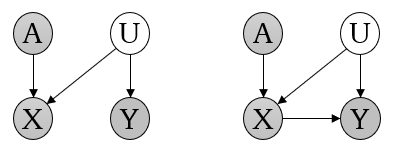
\includegraphics[]{Screenshot 2022-03-04 221940.png}
	\caption{Παραδείγματα αιτιωδών γράφων}
	\label{fig:countfairness}
\end{figure}
\noindent Αναφέραμε τις κυριότερες και πιο γνωστές μετρικές, ωστόσο επειδή τα τελευταία χρόνια έχουν δημιουργηθεί πάρα πολλές μετρικές, δεν είναι δυνατό να αναλυθούν όλες σε αυτή την εργασία. Περισσότερες μετρικές μπορούν να βρεθούν στο \cite{catonFairnessMachineLearning2020}.
\subsection{Διαφάνεια (Transparency) και Λογοδοσία (Accountability)}
\noindent Η λογοδοσία αναφέρεται στο εάν μια απόφαση έχει ληφθεί ακολουθώντας διαδικασίες ενός προτύπου και τον ορισμό ενός υπεύθυνου εάν αυτά τα πρότυπα δεν πληρούνται \cite{krollAccountableAlgorithms}. Εισάγει δηλαδή και την σημασία του ανθρώπινου παράγοντα ως απαραίτητη προϋπόθεση για την αμερόληπτη και σωστή λειτουργία των συστημάτων. Σε αυτή την κατεύθυνση συμβάλλει αρκετά, η αύξηση της διαφάνειας των αλγορίθμων \cite{diakopoulosAccountabilityAlgorithmicDecision2016}. Για τον όρο διαφάνεια τον αλγορίθμων υπάρχουν πολλοί ορισμοί και θεωρήσεις. Ωστόσο αυτό από μόνο του δεν αρκεί. Ο Frank Pasquale στο βιβλίο του ``The black box society" \cite{pasqualeBlackBoxSociety2015} αναφέρεται στο πως οι επιχειρήσεις αλλά και οι κυβερνήσεις συλλέγουν και επεξεργάζονται τεράστιους όγκους δεδομένων, μέσω των οποίων δημιουργούνται εξατομικευμένα προφίλ και λαμβάνονται αποφάσεις για βασικές πτυχές της καθημερινότητας και της ζωής μας, όπως για παράδειγμα η λήψη ενός δανείου ή η επιλογή μαθητών που θα φοιτήσουν σε ένα κολλέγιο \cite{adamsAlevelResultsAlmost2020}, χωρίς να μας δίνουν την δυνατότητα για λεπτομερή έλεγχο της λειτουργίας των αλγορίθμων που επεξεργάζονται τα δεδομένα και λαμβάνουν αποφάσεις. Παράλληλα ο συγγραφέας επισημαίνει, ότι «εχθρός» της διαφάνειας είναι η μεγάλη πολυπλοκότητα. Η λογοδοσία στην τεχνητή νοημοσύνη όμως πέρα από τη διαδικασία λήψης αποφάσεων από έναν αλγόριθμο και τον ορισμό ενός υπεύθυνου για αυτή, σχετίζεται και με την παροχή επεξηγήσεων (explanations). 
\subsection{Ερμηνευσιμότητα (Interpretability) και \\ επεξηγησιμότητα (Explainability)}
\noindent Σε ένα σύστημα μηχανικής μάθησης ένα ζήτημα που υπάρχει είναι ότι τα μοντέλα λειτουργούν σαν ένα μαύρο κουτί (black-box), ειδικά σε ιδιαίτερα περίπλοκα συστήματα όπως είναι τα νευρωνικά δίκτυα. Σύμφωνα με τους Velez και Kim \cite{doshi-velezRigorousScienceInterpretable2017} η ερμηνευσιμότητα (interpretability) ορίζεται ως «η ικανότητα να εξηγήσουμε ένα σύστημα ή να το παρουσιάσουμε με έναν τρόπο που είναι κατανοητός στους ανθρώπους», ενώ πιο ειδικά στον τομέα της τεχνητής νοημοσύνης ερμηνεύσιμο είναι \textit{ένα σύστημα στο οποίο μπορούμε μελετήσουμε και να κατανοήσουμε πως οι είσοδοι αντιστοιχίζονται μαθηματικά στις εξόδους του \cite{doranWhatDoesExplainable2018}}. Πιο συγκεκριμένα, θέλουμε να μάθουμε τι προκάλεσε μια συγκεκριμένη απόφαση που ελήφθη από ένα σύστημα.
Σύμφωνα με τον Molnar \cite{molnarInterpretableMachineLearning2019} οι δύο κύριες κατηγορίες μεθόδων ερμηνευσιμότητας είναι οι αγνωστικές μέθοδοι ως προς το μοντέλο (model-agnostic), στις οποίες διαχωρίζουμε τις εξηγήσεις από το μοντέλο μηχανικής μάθησης, μπορούν να εφαρμοστούν σε οποιοδήποτε μοντέλο μηχανικής μάθησης και εφαρμόζονται μετά την εκπαίδευση του μοντέλου και οι γνωστικές μέθοδοι ως προς το μοντέλο (model-specific) οι οποίες μπορούν να εξηγήσουν μόνο κάποια συγκεκριμένη κλάση μοντέλων.
 Πολλές φορές η έννοια της ερμηνευσιμότητας συγχέεται με την έννοια της επεξηγησιμότητας (explainability). Παράλληλα, αρκετοί είναι οι ορισμοί που έχουν προταθεί για την επεξηγησιμότητα και αρκετές οι διαφορετικές προσεγγίσεις που ακολουθούνται για τη δημιουργία επεξηγήσιμων συστημάτων μηχανικής μάθησης. Ένας, από αυτούς τους ορισμούς στο πεδίο της τεχνητής νοημοσύνης και κατ'επέκταση στο πεδίο της μηχανικής μάθησης δίνεται στο \cite{markusRoleExplainabilityCreating2021}: «Ένα σύστημα τεχνητής νοημοσύνης είναι επεξηγήσιμο εάν είναι εγγενώς ερμηνεύσιμο ή εάν το μη ερμηνεύσιμο μοντέλο εργασίας συμπληρώνεται με μια ερμηνεύσιμη και πιστή εξήγηση (εδώ το σύστημα τεχνητής νοημοσύνης περιέχει επίσης μια εκ των υστέρων (post-hoc) εξήγηση)». Τα μοντέλα που είναι επεξηγήσιμα είναι και ερμηνεύσιμα εξ'ορισμού, όμως το αντίστροφο δεν ισχύει πάντα.

\subsection{Μεροληψία (Bias)} \label{seq:bias}
\noindent Η μεροληψία σχετίζεται άμεσα με την δικαιοσύνη και πολλές φορές τα όρια ανάμεσα σε αυτές τις δύο έννοιες είναι αρκετά δυσδιάκριτα για αρκετούς ανθρώπους.\\
Στο \cite{mehrabiSurveyBiasFairness2021} τα είδη μεροληψίας κατηγοριοποιούνται σύμφωνα με τον βρόχο ανατροφοδότησης που σχηματίζεται στα συστήματα μηχανικής μάθησης ανάμεσα στα δεδομένα, τον αλγόριθμο και τις αλληλεπιδράσεις του χρήστη. Έτσι, διακρίνεται η μεροληψία των δεδομένων τα οποία δίνονται στον αλγόριθμο, η μεροληψία που εισάγεται από τους αλγορίθμους και μπορεί να επηρεάσει τη συμπεριφορά των χρηστών και η μεροληψία που εισάγεται στα δεδομένα από τους χρήστες.
\\\\
\textbf{Τύποι αλγορίθμων μετριασμού μεροληψίας}\\
Οι τεχνικές μετριασμού της μεροληψίας μπορούν να κατηγοριοποιηθούν σε pre-processing, in-processing και post-processing, όπως αναφέρουν οι Caton και Haas \cite{catonFairnessMachineLearning2020}. Οι pre-processing τεχνικές λαμβάνουν χώρα πριν την εκπαίδευση του μοντέλου και προσπαθούν να μετριάσουν την μεροληψία που υπάρχει στα δεδομένα που δίνονται στο μοντέλο για την εκπαίδευσή του. Θεωρείται αρκετά ευέλικτη τεχνική καθώς οι αλγόριθμοι που την χρησιμοποιούν δεν επηρεάζουν καθόλου το μοντέλο που θα χρησιμοποιηθεί. Οι in-processing τεχνικές εφαρμόζονται κατά τη διάρκεια της εκπαίδευσης του μοντέλου και τροποποιούν ήδη υπάρχοντες αλγορίθμους προκειμένου αυτοί να είναι πιο δίκαιοι στις αποφάσεις που παίρνουν. Η τελευταία τεχνική, η post-processing έχει ως στόχο να κάνει πιο δίκαιες τις προβλέψεις που έχει παράξει ένας αλγόριθμος, άρα εφαρμόζεται μετά την εκπαίδευση του μοντέλου, είναι και αυτή αρκετά ευέλικτη τεχνική καθώς είναι ανεξάρτητη από το μοντέλο και δεν χρειάζεται να αποκτήσει πρόσβαση σε αυτό παρά μόνο στα αποτελέσματα. Φυσικά υπάρχει και ο συνδυασμός δύο ή και τριών ειδών.\\\\
Ένα από τα πιο γνωστά και πιο πλήρη ανοικτού κώδικα (open-source) εργαλεία για εύρεση και μετριασμό της μεροληψίας μέσω διάφορων τεχνικών και αλγορίθμων της μεροληψίας, αποτελεί το AI Fairness 360 (AIF360) της IBM \cite{bellamyAIFairness3602018} σε γλώσσα python και R. Το εργαλείο αυτό, περιέχει 71 μετρικές μεροληψίας, 9 αλγορίθμους μετριασμού της μεροληψίας, καθώς και περιγραφή κάθε μετρικής σε γλώσσα απλή και κατανοητή από όλους τους χρήστες. Θα πρέπει να σημειωθεί πως έχουν αναπτυχθεί αρκετά παρόμοια εργαλεία, με τα πιο γνωστά από αυτά να είναι το FairLearn \cite{bird2020fairlearn} της Microsoft και το Aequitas \cite{saleiroAequitasBiasFairness2019} που αναπτύχθηκε από το πανεπιστήμιο του Σικάγο των Η.Π.Α..\\
Είναι γεγονός ότι έως σήμερα έχει διεξαχθεί αρκετά εκτενής έρευνα σχετική με ζητήματα δικαιοσύνης, λογοδοσίας, διαφάνειας και ερμηνευσιμότητας, ενώ αρκετές είναι και οι προσπάθειες για τον μετριασμό της μεροληψίας όπως προαναφέρθηκε, σε διάφορους τομείς της μηχανικής μάθησης (κατηγοριοποίηση, παλινδρόμηση, Graph Embedding/Clustering, εκμάθηση αναπαραστάσεων (representation learning), επεξεργασία φυσικής γλώσσα (NLP) είναι τα κυριότερα). Σε αυτούς τους τομείς ωστόσο δεν συμπεριλαμβάνονται τα Συστήματα συστάσεων (recommender/recommendation systems). Παρόλα αυτά, τα τελευταία χρόνια αρχίζουν και γίνονται αξιόλογες προσπάθειες και σε αυτόν τον τομέα.


\section{Ηθικά ζητήματα στα συστήματα συστάσεων}
\noindent Στο \cite{chenBiasDebiasRecommender2020} παρουσιάζονται διάφορα είδη μεροληψίας που συναντάμε στα συστήματα συστάσεων καθώς και διάφοροι αλγόριθμοι και τεχνικές για τον μετριασμό της. Επιπροσθέτως, παρουσιάζεται ο κύκλος ζωής των συστημάτων συστάσεων ως ένας βρόχος ανατροφοδότησης (feedback loop) ανάμεσα σε τρεις κυρίαρχους παράγοντες: τους χρήστες, τα δεδομένα και το μοντέλο, όπως φαίνεται και στην Εικόνα \ref{fig:feedbackloop}.
\begin{figure}[!htb]
	%\vspace{2px}%
	\centering
	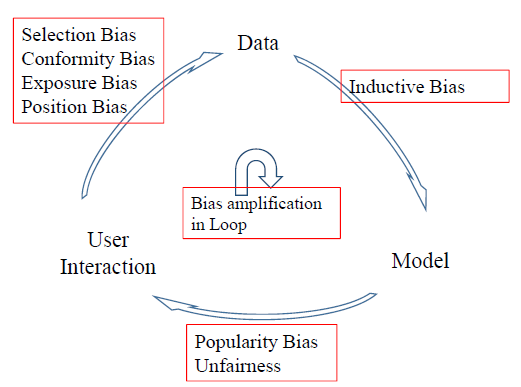
\includegraphics[]{feedbackloop.png}
	\caption[Βρόχος ανατροφοδότησης στα συστήματα συστάσεων]{Βρόχος ανατροφοδότησης στα συστήματα συστάσεων [Πηγή: \url{https://arxiv.org/pdf/2010.03240v1.pdf}]}
	\label{fig:feedbackloop}
\end{figure}
Η μεροληψία στα δεδομένα μπορεί να κατηγοριοποιηθεί περαιτέρω σε μεροληψία στο explicit feedback και στο implicit feedback, δύο έννοιες που είδαμε αναλυτικά στην Ενότητα \ref{rec_sys_chap}. Τα είδη μεροληψίας που παρουσιάζονται συνοπτικά είναι:\\

\noindent\textbf{Μεροληψία επιλογής (Selection Bias)}\\
Η μεροληψία επιλογής, κάνει την εμφάνισή της όταν οι χρήστες είναι ελεύθεροι να επιλέξουν ποια αντικείμενα θα αξιολογήσουν και έτσι οι παρατηρηθείσες αξιολογήσεις (observed ratings) δεν είναι αντιπροσωπευτικό δείγμα όλων των αξιολογήσεων, δηλαδή τα δεδομένα αξιολογήσεων (rating data) συχνά είναι missing not at random (MNAR) το οποίο σημαίνει πως τα δεδομένα λείπουν για λόγους που δεν είναι γνωστοί σε εμάς.\\

\noindent\textbf{Μεροληψία κομφορμισμού (Conformity Bias)}\\
Ο κομφορμισμός είναι μια αρκετά γνωστή έννοια στην επιστήμη της ψυχολογίας και αναφέρεται στην αλλαγή της συμπεριφοράς ενός ατόμου προκειμένου να ταιριάξει με τις συμπεριφορές των ατόμων γύρω του \cite{cialdiniSocialInfluenceCompliance2004}. Στα συστήματα συστάσεων οι χρήστες έχουν την τάση να αξιολογούν αντικείμενα ακολουθώντας τον τρόπο αξιολόγησης των άλλων χρηστών, ακόμη και αν αυτό έρχεται σε αντίθεση με την προσωπική τους κρίση. Για παράδειγμα, αν μια ταινία έχει χιλιάδες αξιολογήσεις και μέσο όρο αξιολόγησης που αγγίζει ή και ξεπερνάει τα 4 στα 5 αστέρια, είναι αρκετά πιθανό να μην το αξιολογήσει αρνητικά ακόμη και αν αυτή ήταν η αρχική του πρόθεση. Αυτό έχει ως συνέπεια οι αξιολογήσεις πολλές φορές να μην αντικατοπτρίζουν την πραγματική κρίση/προτίμηση του χρήστη. To conformity bias φαίνεται πως συνδέεται και με ένα άλλο είδος μεροληψίας το popularity bias (υποενότητα \ref{popularity bias}), καθώς οι χρήστες συνηθίζουν να αλληλεπιδρούν με δημοφιλή αντικείμενα, για παράδειγμα αγοράζουν ένα προϊόν έχοντας ως βασικό κριτήριο τη δημοφιλία του, δηλαδή τον αριθμό των πωλήσεων ή των αξιολογήσεων του \cite{zhengDisentanglingUserInterest2021a}.\\

\noindent\textbf{Μεροληψία έκθεσης (Exposure Bias)}\\
Αυτό το είδος μεροληψίας συμβαίνει καθώς οι χρήστες εκτίθενται μόνο σε ένα μέρος των αντικειμένων μιας λίστας και εξαιτίας αυτού οι μη παρατηρηθείσες αλληλεπιδράσεις (unobserved interactions) δεν αντιπροσωπεύουν πάντα αρνητική προτίμηση. Με άλλα λόγια, αν ένας χρήστης δεν έχει δει ένα αντικείμενο δεν μπορεί να προκύψει το αυθαίρετο συμπέρασμα ότι δεν του αρέσει αυτό το αντικείμενο. Οι ερευνητές έχουν εξετάσει από διάφορες οπτικές αυτό το είδος μεροληψίας. Μια εξ αυτών θεωρεί πως το popularity bias είναι μια μορφή μεροληψίας έκθεσης, διότι το τμήμα των αντικειμένων στο οποίο εκτίθεται περισσότερο ένας χρήστης είναι τα δημοφιλή αντικείμενα. Ενώ μια άλλη, σχετίζεται με την αναζήτηση που πραγματοποιούν οι χρήστες προκειμένου να βρουν τα αντικείμενα που τους ενδιαφέρουν και την επιλογή αυτών. Η επιλογή αυτή θεωρείται ως ένας τύπος έκθεσης, ο οποίος δίνει αρκετά περισσότερες πιθανότητες στα πολύ σχετικά αντικείμενα να προβληθούν/εκτεθούν και επομένως το exposure bias μπορεί να ονομαστεί αλλιώς και selection bias. 
\newpage
\noindent\textbf{Μεροληψία θέσης (Position Bias)}\\
Σχετίζεται με την τάση των ανθρώπων να αλληλεπιδρούν με αντικείμενα τα οποία βρίσκονται στις πιο υψηλές θέσεις των λιστών συστάσεων (recommendation lists) ανεξάρτητα από την πραγματική σχετικότητα των αντικειμένων αυτών. To position bias θεωρείται πως είναι ένας τύπος selection bias. Ένα χαρακτηριστικό παράδειγμα αυτού αποτελούν τα βίντεο που μας προτείνει το YouTube. Ένας χρήστης συνήθως θα επιλέξει να παρακολουθήσει κάποιο από τα πρώτα βίντεο που του προτείνει αγνοώντας όσα είναι πιο χαμηλά στη λίστα, τα οποία όμως μπορεί να είναι πιο ενδιαφέροντα και πιο σχετικά με τις προτιμήσεις του.\\


\noindent\textbf{Μεροληψία συναισθήματος (Sentiment bias)}\\
Στο \cite{linMitigatingSentimentBias2021} ορίζεται ένας ακόμη τύπος μεροληψίας, η μεροληψία συναισθήματος ως «\textit{η απόκλιση μεταξύ της απόδοσης των συστημάτων συστάσεων σε χρήστες/στοιχεία με θετικό feedback και σε χρήστες/στοιχεία με αρνητικό feedback}». Πιο αναλυτικά, τα συστήματα συστάσεων κάνουν αρκετά πιο ακριβείς προτάσεις σε χρήστες/αντικείμενα που έχουν θετικό feedback (positive feedback) σε σχέση με χρήστες/αντικείμενα που έχουν αρνητικό feedback (negative feedback). Συνέπεια αυτού είναι τόσο η χαμηλή ποιότητα στις συστάσεις που προσφέρονται στους χρήστες, όσο και μη δίκαιη εκπροσώπηση των αντικειμένων που λαμβάνουν θετικά σχόλια από ένα μικρό μέρος του πληθυσμού (τα λεγόμενα και niche items). Αξίζει να σημειωθεί πως αυτό το είδος μεροληψίας αν και εκ πρώτης όψεως μοιάζει να έχει αρκετά κοινά με άλλη είδη, όπως για παράδειγμα με το popularity bias, εντούτοις είναι διαφορετικό.\\

\noindent Στις επόμενες δύο υποενότητες αναλύονται εκτενέστερα, η μεροληψία που εισάγει το μοντέλο στα αποτελέσματα που παράγει και δίνει στους χρήστες λόγω της σημαντικότητάς τους. Πιο συγκεκριμένα, αναλύονται: η έννοια της δικαιοσύνης στα αποτελέσματα που παράγει ένα σύστημα συστημάτων συστάσεων, ενώ παράλληλα περιγράφονται τα πιο σημαντικά είδη αυτής, και ένα πολύ σοβαρό είδος μεροληψίας, το popularity bias.

\subsection{Δικαιοσύνη}
\noindent O Yao στο \cite{NIPS2017_e6384711}  παρουσιάζει μορφές αδικίας (unfairness) που υπάρχουν στα μοντέλα συνεργατικής διήθησης. Πιο συγκεκριμένα, περιγράφει μια διαδικασία μέσω της παραγοντοποίησης μητρώου, η οποία οδηγεί σε άδικες συστάσεις (unfair recommendations) - δηλαδή συστάσεις που εισάγουν κάποιο είδος μεροληψίας -, ακόμη και όταν τα δεδομένα αξιολογήσεων αντικατοπτρίζουν με ακρίβεια τις προτιμήσεις των χρηστών. Αυτού του είδους το unfairness, προκύπτει από την ελλιπή εκπροσώπηση (underrepresentation). Ανιχνεύτηκαν, 2 μορφές αυτής: η άνιση κατανομή πληθυσμιακών ομάδων (Population imbalance) και η μεροληψία παρατήρησης (observation bias) η οποία είναι αρκετά παρόμοια με την μεροληψία έκθεσης που περιγράψαμε στην προηγούμενη υποενότητα.\\
Στο \cite{liCIKM2021Tutorial2021} η διάκριση των τύπων δικαιοσύνης στα συστήματα συστάσεων είναι η εξής: ατομική/ομαδική, στατική/δυναμική, μονόπλευρη/πολύπλευρη, αντικειμένου/χρήστη και συνειρμική/αιτιώδης.\\
Όπως και σε άλλα πεδία της μηχανικής μάθησης και στα συστήματα συστάσεων υπάρχει η διάκριση μεταξύ ομαδικής (Group) και ατομικής (Individual) δικαιοσύνης.\\
Στο \cite{burkeMultisidedFairnessRecommendation2017} ορίζονται τα εμπλεκόμενα μέρη στα συστήματα συστάσεων: \begin{itemize}
	\item \textbf{οι καταναλωτές (consumers - C)}, δηλαδή εκείνοι που δέχονται τις προτάσεις
	\item \textbf{οι πάροχοι (providers - P)}, δηλαδή εκείνοι που έχουν κάποιο κέρδος από τις επιλογές του καταναλωτή και υποστηρίζουν (χορηγούν) τα προτεινόμενα αντικείμενα 
	\item \textbf{η πλατφόρμα ή αλλιώς το σύστημα (System – S)} που δημιουργεί τις συστάσεις.
\end{itemize} Σύμφωνα με αυτή την κατηγοριοποίηση ορίζονται αντίστοιχα οι έννοιες και στο fairness: C-fairness, P-fairness και CP-fairness. Οι δύο πρώτες έννοιες, εντάσσονται στην κατηγορία της δικαιοσύνης που ονομάζεται μονόπλευρη (single-sided fairness) καθώς εξετάζει την ύπαρξη δίκαιων αποτελεσμάτων μόνο για την μία πλευρά. Αντίθετα η περίπτωση της CP-fairness, στην οποία λαμβάνεται υπόψη τόσο η δικαιοσύνη από την πλευρά του καταναλωτή, όσο και από την πλευρά του παρόχου, ανήκει στην ευρύτερη κατηγορία της πολύπλευρης δικαιοσύνης (multi-sided fairness). Έκτοτε, στην βιβλιογραφία συναντάμε αρκετές μετρικές που ανήκουν σε μια από τις προαναφερθείσες κατηγορίες. \\
Η συνειρμική δικαιοσύνη (Associative Fairness) αναφέρεται στην απόκλιση των στατιστικών μετρικών μεταξύ ατόμων ή υποπληθυσμών. Οι περισσότερες έννοιες δικαιοσύνης στα συστήματα συστάσεων που συναντάμε στη βιβλιογραφία βασίζονται σε αυτή τη θεώρηση. Μία διαφορετική θεώρηση από αυτή αποτελεί η αιτιώδης δικαιοσύνη (Causal Fairness). Μια από τις πρώτες προσπάθειες, αν όχι η πρώτη, είναι η τεχνική που παρουσιάζεται στο \cite{liPersonalizedFairnessBased2021} για την οποία δημιουργήθηκαν αιτιώδεις γράφοι (causal graphs) για να περιγραφεί το πως επηρεάζουν τα προστατευόμενα χαρακτηριστικά τη δημιουργία των συστάσεων. \\
Μια άλλη θεώρηση είναι η δικαιοσύνη για τον χρήστη (User Fairness) και η δικαιοσύνη για το αντικείμενο (Item Fairness). Η δικαιοσύνη για τον χρήστη αναφέρεται στην μεροληψία που εισάγεται κατά την παραγωγή συστάσεων για ορισμένους χρήστες ή (συχνότερα) ομάδες χρηστών και η δικαιοσύνη για το αντικείμενο σχετίζεται με την δικαιοσύνη που πρέπει να υπάρχει στα αντικείμενα που προτείνονται. Χαρακτηριστικότερο παράδειγμα στο οποίο εξετάζεται η δικαιοσύνη για τα αντικείμενα είναι το popularity bias, που αναλύεται λεπτομερώς στην αμέσως επόμενη υποενότητα. \\
Μια ακόμη έννοια που συναντάμε είναι αυτή της στατικής δικαιοσύνης. Στατική δικαιοσύνη (Static fairness) σημαίνει ότι τα προστατευόμενα χαρακτηριστικά ή οι ετικέτες των ομάδων (group labels), όπως για παράδειγμα το φύλο και ηλικία, είναι σταθερά σε όλη την κατάταξη ή τη διαδικασία δημιουργίας συστάσεων. Αντίθετα, η δυναμική δικαιοσύνη
(Dynamic fairness) \cite{geLongtermFairnessRecommendation2021} λαμβάνει υπόψη της τους δυναμικούς παράγοντες στο περιβάλλον των συστημάτων συστάσεων. Αυτοί εμπεριέχουν τις αλλαγές στη χρησιμότητα ή τα χαρακτηριστικά των αντικειμένων σε αυτό το περιβάλλον. Αφού γίνει αυτό σειρά έχει η εκμάθηση μιας στρατηγικής για να ανταποκρίνεται το σύστημα σε τέτοιες δυναμικές.\\
Στο \cite{elahiAlgorithmicFairnessRecommender2021} παρουσιάζεται μια αρκετά διαφορετική κατηγοριοποίηση της δικαιοσύνης, η οποία δεν εντάσσεται στο πλαίσιο της δικαιοσύνης που σχετίζεται με τους αλγορίθμους, όπως όσες προαναφέρθηκαν και όσες αναφέρονται στη βιβλιογραφία. Πιο συγκεκριμένα, διακρίνονται τρεις μορφές δικαιοσύνης.\\
 Πρώτα παρουσιάζεται η δικαιοσύνη στην αφοσίωση του χρήστη (Engagement), η οποία σχετίζεται με το πώς διαφορετικοί χρήστες δεσμεύονται και παρακινούνται να χρησιμοποιούν το σύστημα και να αλληλεπιδρούν
με τις συστάσεις. Ακολούθως, παρουσιάζεται η δικαιοσύνη αναπαράστασης (Representation)  η οποία αφορά την παροχή πολλαπλών μέσων
εκπροσώπησης για τους χρήστες με στόχο την ενίσχυση διαφορετικών χρηστών, οι οποίοι έχουν τις δικές τους συγκεκριμένες φυσικές και γνωστικές ικανότητες, για την καλύτερη κατανόηση των  συστάσεων που τους παρουσιάζονται. Ένα παράδειγμα που μπορεί να δοθεί για αυτό ώστε να γίνει πιο κατανοητό, είναι ένας χρήστης με προβλήματα όρασης. Τέλος, ορίζεται η δικαιοσύνη δράσης και έκφρασης (Action \& Expression) όπου το σύστημα θα πρέπει να δίνει τον έλεγχο στον χρήστη ως προς το πώς θέλει να μεταβάλλονται οι συστάσεις και θα πρέπει επίσης να παρέχει πολλαπλά μέσα αλληλεπίδρασης για τους χρήστες.
\noindent \subsection{Μεροληψία δημοφιλίας (Popularity bias)}\label{popularity bias}
\noindent Στην παρούσα εργασία από όλα τα είδη μεροληψίας που συναντάμε στα συστήματα συστάσεων και περιγράφονται σε αυτή την ενότητα, αυτό που θα μας απασχολήσει είναι το popularity bias καθώς φαίνεται πως είναι το πιο σοβαρό και έχει δημιουργήσει πολυάριθμα και σημαντικά προβλήματα. Το φαινόμενο αυτό \textit{περιγράφει την τάση των συστημάτων συστάσεων να προτείνουν τα πιο δημοφιλή αντικείμενα (εκείνα με τις περισσότερες αξιολογήσεις) πολύ πιο συχνά από τα λιγότερο δημοφιλή αντικείμενα, τα λεγόμενα long tail αντικείμενα, που στην μεγάλη πλειονότητα των περιπτώσεων είναι πολύ περισσότερα \cite{parkLongTailRecommender2008}}. 
\begin{figure}[H]
	%\vspace{2px}%
	\centering
	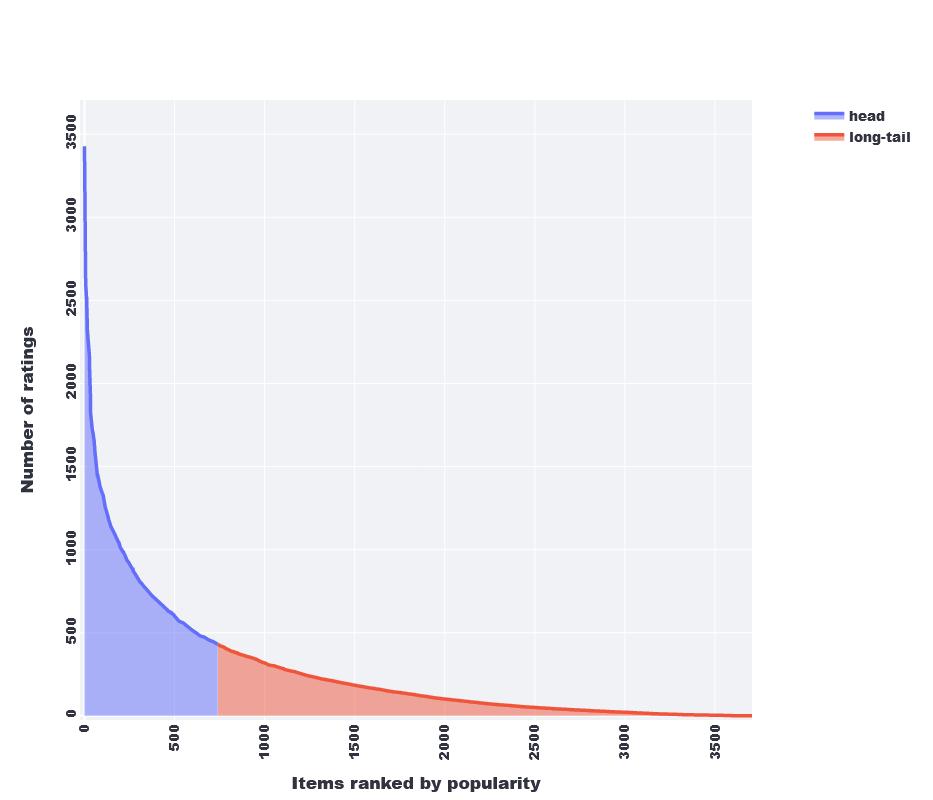
\includegraphics[width=\linewidth]{newplot.png}
	\caption{Διάγραμμα long tail}
	\label{fig:longtail}
\end{figure}
\noindent Ο Chris Anderson στο βιβλίο του ``The Long Tail: Why the Future of Business Is Selling Less of More" \cite{andersonLongTailWhy2006} εισάγει για πρώτη φορά τον όρο “long tail”, ο οποίος βασίζεται στην «αρχή του Pareto» (Pareto Principle), για να περιγράψει το φαινόμενο στο οποίο οι επιχειρήσεις αποκομίζουν σημαντικά κέρδη από την πώληση προϊόντων με χαμηλή ζήτηση ή χαμηλές πωλήσεις σε πολλούς πελάτες, σε σχέση με αυτά που αποκομίζουν από την πώληση μόνο μεγάλων ποσοτήτων ενός περιορισμένου αριθμού δημοφιλών προϊόντων. Η Αρχή του Pareto (Pareto Principle), γνωστή και ως κανόνας του 80/20 ορίζει ότι το 80\% των επιπτώσεων προέρχεται από το 20\% των αιτιών. Στον χώρο των επιχειρήσεων αυτό μεταφράζεται ως: το 20\% των προϊόντων αντιπροσωπεύει το 80\%  των πωλήσεων. Αυτό το 20\% των πιο δημοφιλών προϊόντων ονομάζεται ``head" και το υπόλοιπο 80\% ``long tail", καθώς φαίνεται σαν μια μακριά ουρά, κάτι που είναι ευδιάκριτο στην Εικόνα \ref{fig:longtail}.
Προκειμένου να γίνει πιο κατανοητό το long tail παρατίθεται το παρακάτω γράφημα (Εικόνα \ref{fig:longtail}), το οποίο είναι στο σύνολο δεδομένων Movielens1M που περιέχει αξιολογήσεις ταινιών. Στον άξονα x βρίσκονται τα IDs των ταινιών ταξινομημένα κατά φθίνουσα σειρά, ως προς τον αριθμό των αξιολογήσεων που έχουν λάβει και στον άξονα y ο συνολικός αριθμός των αξιολογήσεων.

 \noindent Ωστόσο, το γεγονός ότι ένα αντικείμενο είναι δημοφιλές δεν σημαίνει αυτομάτως ούτε πως είναι ποιοτικό ούτε ηθικό. Επιπρόσθετα, το popularity bias έχει αποδειχθεί ότι συνδέεται και με άλλους τύπους μεροληψίας και επίσης συμβάλλει στη δημιουργία των φαινομένων “echo chambers” και “filter bubbles”.\\
 Στο φαινόμενο που έχει γίνει γνωστό ως «θάλαμος αντήχησης» (echo chamber) \cite{sunsteinEchoChambersBush2001}, ένα άτομο ή μια ομάδα ατόμων δημιουργούν ένα περιβάλλον μέσα στο οποίο συναντούν μόνο πληροφορίες ή απόψεις που αντανακλούν ή ενισχύουν τις δικές τους, χωρίς να συναντούν αντίθετες απόψεις. 
Το φαινόμενο «φυσαλίδες πληροφορίας» (filter bubbles) πολλές φορές συγχέεται με το echo chambers αν και πρόκειται για κάτι διαφορετικό. Πιο αναλυτικά, στο φαινόμενο filter bubbles οι αλγόριθμοι προτείνουν στους ανθρώπους περιεχόμενο παρόμοιο με τα ενδιαφέροντά τους ή σύμφωνα με τα χαρακτηριστικά τους και το προφίλ τους (παλιά κλικ, ιστορικό αναζήτησης κτλ.), αποκόπτοντας τους έτσι από μεγάλο μέρος του διαθέσιμου περιεχομένου και δημιουργώντας μια «φούσκα» η οποία μειώνει κατά πολύ την ποικιλία (diversity).\\
Εξαιτίας αυτής της μεροληψίας, έχει παρατηρηθεί επίσης το φαινόμενο μεγάλες εταιρίες να πληρώνουν χρήστες προκειμένου να παρέχουν υψηλές αξιολογήσεις και θετικές κριτικές στα προϊόντα τους \cite{ramosNegativeImpactSocial2020}. Επιπρόσθετα, μπορεί να οδηγήσει σε χειραγώγηση των χρηστών από ψεύτικες κριτικές (fake reviews), των bots που συναντάμε στα μέσα κοινωνικής δικτύωσης (social bots ή social media bots) \footnote{\textbf{Social bot:} αλγόριθμος που παράγει αυτόματα περιεχόμενο και αλληλεπιδρά με τους ανθρώπους στα
	μέσα κοινωνικής δικτύωσης, προσπαθώντας να μιμηθεί και
	ενδεχομένως να αλλάξει τη συμπεριφορά τους.\cite{ferraraRiseSocialBots2016} } και στο φαινόμενο που έχει γίνει γνωστό ως “astroturfing", καθώς και στην έλλειψη ανεξαρτησίας και κοινωνικής επιρροής ανάμεσα στα μέλη ενός πλήθους ανθρώπων - όπως αυτό υπονοείται έμμεσα από τη διαθεσιμότητα των ταξινομήσεων (rankings) - η οποία υπονομεύει σοβαρά την αξιοπιστία των σημάτων ένδειξης της δημοφιλίας (popularity signals), όπως αναφέρει ο Ciampaglia στο  \cite{ciampagliaHowAlgorithmicPopularity2018}. Χρησιμοποιώντας τον όρο ``astroturfing", αναφερόμαστε στην προσπάθεια να δημιουργηθεί μια εντύπωση ευρείας υποστήριξης από τη βάση για μια πολιτική, άτομο ή προϊόν, όπου στην πραγματικότητα υπάρχει μικρή τέτοια υποστήριξη. Με αυτόν τον τρόπο στα μέσα κοινωνικής δικτύωσης προωθούνται πολλές φορές ακραίες, ψευδείς ή ακόμα και επικίνδυνες αναρτήσεις   οι οποίες μπορούν να διαβρώσουν και να αλλοιώσουν μια κοινωνία, να προωθήσουν τον εξτρεμισμό και την βία, ή ακόμα και να οδηγήσουν σε αλλοίωση των πολιτικών αποτελεσμάτων ή ακόμα χειρότερα σε εμπόλεμες διαμάχες. Πρόσφατες έρευνες δείχνουν πως τα μέσα κοινωνικής δικτύωσης ευθύνονται για την διάδοση ψευδών ειδήσεων σχετικών με την πανδημία της COVID-19 και τα εμβόλια για διάφορες ασθένειες, αποτρέποντας τους ανθρώπους να εμβολιαστούν, αυξάνοντας έτσι τον αριθμό των θανάτων και την πίεση στο εθνικό σύστημα υγείας. Καθοριστικό ρόλο σε αυτή τη διάδοση φαίνεται πως διαδραματίζουν οι αλγόριθμοι των συστημάτων συστάσεων. Εκτός όμως από τα μέσα κοινωνικής δικτύωσης,  popularity bias συναντάμε σχεδόν παντού πλέον στο διαδίκτυο, από τις ιστοσελίδες που χρησιμοποιούμε για την ψυχαγωγία μας  και τις αγορές μας, μέχρι και εκείνες που χρησιμοποιούμε για την εύρεση εργασίας   και την αναζήτηση πηγών για επιστημονική έρευνα. Στο \cite{borattoEffectAlgorithmicBias2019} γίνεται έρευνα σχετικά με την επίδραση του popularity bias στα Massive Open Online Courses (MOOC’s). Καθίσταται επομένως επιτακτική η ανάγκη να εξαλείψουμε  τη μεροληψία αυτού του είδους των αλγορίθμων.\\

\noindent \textbf{Αλγόριθμοι μετριασμού μεροληψίας}\\
Σε αυτήν την υποενότητα παρουσιάζονται ορισμένοι από τους πιο σημαντικούς αλγορίθμους και τεχνικές για τον μετριασμό της μεροληψίας, που ανήκουν στις τρεις κατηγορίες που αναφέραμε στην υποενότητα \ref{seq:bias}: pre-processing, in-processing και post-processing. Ιδιαίτερη έμφαση δίνεται στην post-processing κατηγορία, διότι αυτή χρησιμοποιήθηκε κατά κύριο λόγο σε αυτή την εργασία, ενώ θα πρέπει να σημειωθεί πως περιγράφονται αναλυτικά μόνο οι αλγόριθμοι που χρησιμοποιήθηκαν στα πειράματά μας.\\

\noindent \textbf{Pre-processing}\\
Στο \cite{rastegarpanahFightingFireFire2019} η τεχνική που προτείνεται αφήνει το σύνολο εκπαίδευσης ανέγγιχτο και απλά προσθέτει σε αυτό δεδομένα που τα ονομάζει «αντίδοτο», καθώς αποτελούν ένα «αντίδοτο» στην μεροληψία που περιέχουν τα δεδομένα. Αυτή η τεχνική που εφαρμόζεται σε έναν αλγόριθμο παραγοντοποίησης μητρώου στον οποίο έχει γίνει η εκπαίδευση δίνοντας του ως είσοδο τα δεδομένα που επιθυμούμε, προσθέτουμε «ψεύτικους» χρήστες και μαζί ψεύτικες αξιολογήσεις που έχουν πραγματοποιήσει. Αυτές οι νέες αξιολογήσεις είναι στην ουσία τα δεδομένα αντιδότου.\\


\noindent \textbf{In-processing}\\
Μια προσέγγιση σε αυτή την κατηγορία είναι η προσθήκη όρων κανονικοποίησης στη συνάρτηση απώλειας (loss function) του μοντέλου. Μέσω αυτών των όρων γίνεται η ρύθμιση της μεροληψίας που εισάγεται. O αλγόριθμος που πρότεινε ο Kamishima στο \cite{kamishimaRecommendationIndependence2018} έχει ως στόχο την στατιστική ανεξαρτησία, δηλαδή να μην συμπεριλάβει οτιδήποτε αφορά το προστατευόμενο χαρακτηριστικό που να επηρεάζει το αποτέλεσμα. Η τεχνική που παρουσιάζεται στο \cite{borgesEnhancingLongTerm2019} βασίζεται στην τεχνική των Variational Autoencoders (VAE) \cite{liangVariationalAutoencodersCollaborative2018a} στη συνεργατική διήθηση. Σε αυτή αποδεικνύεται πως ο θόρυβος στην κανονική κατανομή και στην κατανομή Gauss κατά τη φάση δοκιμής των VAE αλλάζει τα scores του αποτελέσματος, όταν έχουν τα ίδια δεδομένα ως είσοδο και μπορεί να μειώσει το unfairness, αν και οδηγεί σε μια μικρή μείωση της ακρίβειας. \\

\noindent \textbf{Post-processing}\\
Η πιο γνωστή τεχνική σε αυτή την κατηγορία είναι η τεχνική του re-ranking (ανακατάταξη). Σε αυτή, οι αλγόριθμοι παίρνουν ως είσοδο την αρχική λίστα συστάσεων που έχει δημιουργήσει ο αρχικός (base) αλγόριθμος, την επεξεργάζονται και δίνουν ως έξοδο μια λίστα μικρότερου μεγέθους από την αρχική.
Στο \cite{liuPersonalizingFairnessawareReranking2018} οι Liu και Burke πρότειναν δύο re-ranking αλγορίθμους τον \textit{Fairness-Aware Re-ranking (FAR)} και τον \textit{Personalized Fairness-Aware Re-ranking (PFAR)}, οι οποίοι βασίζονται στον αλγόριθμο eXplicit Query
Aspect Diversification (xQuAD) \cite{santosExploitingQueryReformulations2010}. Με τη χρήση αυτών των αλγορίθμων διασφαλίζεται ότι αντικείμενα από διαφορετικές κατηγορίες, όπως είναι η long tail και η head λαμβάνουν μια δίκαιη έκθεση στη λίστα συστάσεων.
\begin{figure}[!htb]
	%\vspace{2px}%
	\centering
	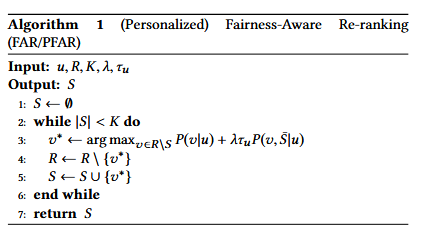
\includegraphics[]{far_pfar.png}
	\caption[Οι αλγόριθμοι FAR και PFAR] {Οι αλγόριθμοι FAR και PFAR [Πηγή: \url{https://arxiv.org/pdf/1809.02921.pdf}
		]}
	\label{fig:far_pfar}
\end{figure}
 Έστω R μια λίστα συστάσεων η οποία έχει παραχθεί από έναν base αλγόριθμο συστάσεων, u είναι ένας χρήστης, S η re-ranked λίστα συστάσεων, K ο αριθμός των αντικειμένων που θα περιέχει η S, $ \lambda\in\left(0,\ 1\right) $ μια παράμετρος η οποία ελέγχει το ποσοστό δικαιοσύνης του παρόχου, $  \tau_u $ είναι ένα εξατομικευμένο βάρος (personalized weight) του οποίου η εκμάθηση γίνεται από το ιστορικό της συμπεριφοράς κάθε χρήστη. Αν $ \tau_u\ = 1 $ τότε έχουμε τον αλγόριθμο FAR, ενώ αν $ \tau_u $ είναι μια τιμή εξατομικευμένου βάρους του οποίου έχει γίνει η εκμάθηση (personalized learned value) τότε έχουμε τον αλγόριθμο PFAR.
\begin{align*}
 \underset{\substack {v\in R(u)}}{max}\underbrace { (1-\lambda) P\left(v\middle| u\right)}_{\text {personalization}} + \underbrace{\lambda \textcolor{red}{\tau_u} \sum_c{PV_c} \mathbb{1}_{\left\{v\in V_c\right\}}\ \prod_{i\in S(u)}\mathbb{1}_{i\not\in V_c}} _{\text {fairness}}
\end{align*}
Όπου $ P\left(v\middle| u\right)  $ είναι η πιθανότητα ενός χρήστη $  u\in U $ να ενδιαφέρεται για το αντικείμενο $ v\in V $, η οποία έχει προβλεφθεί από τον base αλγόριθμο συστάσεων. Στην Εικόνα \ref{fig:far_pfar} παρατίθεται αναλυτικά ο αλγόριθμος FAR/PFAR όπως αυτός παρουσιάστηκε στο \cite{liuPersonalizingFairnessawareReranking2018}.\\
Μια ακόμη γνωστή τεχνική είναι αυτή που περιγράφεται μέσω του αλγορίθμου\textit{ Calibrated recommendations} (Cali) \cite{steckCalibratedRecommendations2018}
όπου κατατάσσουμε εκ νέου τις προτάσεις που παρέχουμε στους χρήστες, για να διασφαλίσουμε την πληρέστερη αντιστοίχιση της κατανομής των ενδιαφερόντων του χρήστη στα χαρακτηριστικά των στοιχείων. Στο σημείο αυτό ας δούμε με περισσότερη λεπτομέρεια πως λειτουργεί αυτός ο αλγόριθμος. Έστω δύο κατανομές, η κατανομή πάνω στα είδη g των αντικειμένων, του συνόλου αντικειμένων H με τα οποία έχει αλληλεπιδράσει ο χρήστης u στο παρελθόν:
\begin{align}
	p(g|u) = \sum_{i \in H} p(g|i)
\end{align}
και η κατανομή πάνω στα είδη των αντικειμένων g, του συνόλου των αντικειμένων I που προτείνονται στον χρήστη u.
\begin{align}
	q(g|u) = \sum_{i \in I} p(g|i)
\end{align}
Ωστόσο δεν είναι λίγες οι φορές όπου τα αντικείμενα που προτείνονται σε έναν χρήστη δεν προσαρμόζονται κατάλληλα σύμφωνα με τις αλληλεπιδράσεις του στο παρελθόν. Προκειμένου να λυθεί αυτό το πρόβλημα χρειαζόμαστε μια μετρική ρύθμισης/προσαρμογής (calibration metric) C. Για την σύγκριση των δύο κατανομών και την μέτρηση της ομοιότητάς τους υπάρχουν αρκετές μέθοδοι, με την πιο δημοφιλή από αυτές να είναι η απόκλιση (divergence) Kullback-Leibler(KL):
\begin{align}
	C(p,q) = D_{KL}(p || q) = \sum_{g} p(g|u) \cdot \log \frac{p(g|u)}{\tilde{q}(g|u)}
\end{align}
Στην περίπτωση που $ q(g|u) = 0 $ και $ p(g|u) > 0 $ για ένα είδος g, τότε:
\begin{align}
	\tilde{q}(g|u) = (1 - \alpha) \cdot q(g|u) + \alpha \cdot p(g|u)
\end{align}
για την εφαρμογή του calibration ο αλγόριθμος λαμβάνει ως είσοδο μια λίστα συστάσεων την οποία ανακατατάσσει, λειτουργώντας ακριβώς όπως ένας post-processing αλγόριθμος. Ο υπολογισμός του βέλτιστου συνόλου $ I^* $ των αντικειμένων που θα προταθούν δίνεται από την σχέση μέγιστης οριακής συνάφειας (maximum marginal relevance):
\begin{align}
	I^* = \underset{I, |I|=N}{\text{argmax}} \; (1 - \lambda) \cdot s(I) - \lambda \cdot C_{KL}(p, q(I))
\end{align}
όπου $ s(i) $ είναι η βαθμολογία (score) των αντικειμένων $ i \in I $ που έχει προβλεφθεί από το σύστημα συστάσεων, $ s(I) = \sum_{i \in I} s(i) $, το άθροισμα των βαθμολογιών όλων των αντικειμένων στη λίστα συστάσεων και $ \lambda \in [0, 1] $ είναι μια παράμετρος ρύθμισης που καθορίζει την αντιστάθμισμα (trade-off) ανάμεσα στη βαθμολογία που έχει δημιουργηθεί από το σύστημα συστάσεων και από την βαθμολογία του calibration score. Μια παρατήρηση εδώ είναι πως επειδή η μέτρηση του calibration score γίνεται από την KL-divergence, στον τύπο της χρησιμοποιούμε το αρνητικό μιας και είναι μια μετρική όπου όσο χαμηλότερη είναι η τιμή της τόσο το καλύτερο.
\\
Ο αλγόριθμος \textit{FA*IR} \cite{zehlikeFAIRFair2017} δημιουργεί ουρές αντικειμένων που ανήκουν σε προστατευόμενες ομάδες και αντικειμένων που δεν ανήκουν και επιλέγει από κάθε ουρά για να δημιουργήσει την τελική re-ranked λίστα. Ας δούμε λίγο πιο αναλυτικά πώς λειτουργεί ο συγκεκριμένος αλγόριθμος.\\ Έστω $ \left[ n \right] =\left\lbrace 1, 2, \dots ,n \right\rbrace  $ ένα σύνολο υποψηφίων (candidates) και έστω $ q_i $ για $ i \in \left[n \right]  $ η «ποιότητα» του υποψηφίου i. Υπάρχουν δύο είδη υποψηφίων, εκείνοι που ανήκουν σε μια προστατευόμενη ομάδα και εκείνοι που δεν ανήκουν σε κάποια προστατευμένη ομάδα. Εάν ανήκουν σε μια προστατευόμενη ομάδα τότε $ q_i = 1 $, αλλιώς  $ q_i = 0 $. Σε μια κατάταξη αντικειμένων μεγέθους k που έχει δοθεί ως είσοδος, συγκρίνεται \textit{σε κάθε θέση της κατάταξης} ο αριθμός των αντικειμένων που ανήκουν σε μια προστατευόμενη ομάδα σε σχέση με τον αναμενόμενο αριθμό των αντικειμένων που ανήκουν σε μια προστατευόμενη ομάδα αν αυτά επιλέγονταν τυχαία με χρήση δοκιμών Bernoulli. Ο αριθμός αυτός, δεν θα πρέπει να είναι μικρότερος από την ελάχιστη ποσότητα $ p $. Μαθηματικά αυτό μεταφράζεται σε μία αθροιστική συνάρτηση διωνυμικής κατανομής F με παραμέτρους $  p, k $ και $ α $:
$ F(\tau _p; k, p) > \alpha , $ όπου $ \tau _p  $ είναι ο πραγματικός αριθμός των προστατευόμενων αντικειμένων στην κατάταξη και $ \alpha $ μια παράμετρος σημαντικότητας η οποίας μας δίνει την πιθανότητα να απορρίψουμε μια δίκαιη κατάταξη. Η προσαρμοσμένη σημαντικότητα $ \alpha_c = c\left(a, k, p \right) $, χρησιμοποιείται διότι ελέγχει πολλαπλές υποθέσεις, καθώς αν χρησιμοποιήσουμε $ \alpha_c = \alpha $ υπάρχει πιθανότητα να δημιουργηθούν πολλά ψευδώς αρνητικά.\\
Ο αλγόριθμος παίρνει ως είσοδο τον αριθμό των αντικειμένων που θα περιέχει η λίστα κατάταξης για κάθε χρήστη, έναν πίνακα που αντιστοιχίζει κάθε αντικείμενο που υπάρχει στο σύνολο δεδομένων με το αν αυτό ανήκει σε προστατευόμενη ομάδα ή όχι (long tail ή head στην περίπτωσή μας), τo προσαρμοσμένο επίπεδο σημαντικότητας $ \alpha_c $ και την ελάχιστη ποσότητα $ p $ των υποψηφίων που ανήκουν σε κάποια προστατευόμενη ομάδα. \\
Αρχικά, ο FA*IR δημιουργεί δύο ουρές προτεραιότητας με έως και k υποψηφίους η κάθε μια, τις $ P_0 $ και $ P_1 $ για τα αντικείμενα για τα αντικείμενα που δεν ανήκουν σε κάποια προστατευόμενη ομάδα και για τα αντικείμενα που ανήκουν, αντίστοιχα. Στην συνέχεια, δημιουργεί έναν πίνακα \textit{m} ο οποίος σε κάθε γραμμή περιέχει τον ελάχιστο αριθμό των υποψηφίων που ανήκουν στην προστατευόμενη ομάδα σε κάθε μία από τις κορυφαίες k (top k) θέσεις ώστε να ικανοποιείται το κριτήριο, κάθε στήλη του πίνακα περιέχει μια συγκεκριμένη τιμή του k. Αν ο πίνακας m απαιτεί έναν υποψήφιο που ανήκει σε μια προστατευόμενη ομάδα  στη συγκεκριμένη θέση τότε ο αλγόριθμος τοποθετεί τον καλύτερο υποψήφιο από την ουρά $ P_1 $ στην κατάταξη, αλλιώς τοποθετεί τον καλύτερο υποψήφιο από την ένωση των 2 ουρών $ P_0 \cup P_1 $.\\
% $\mathcal{O}(n + k\log k) $

\noindent \textbf{Συνδυασμός τεχνικών}\\
\begin{figure}[H]
	%\vspace{2px}%
	\centering
	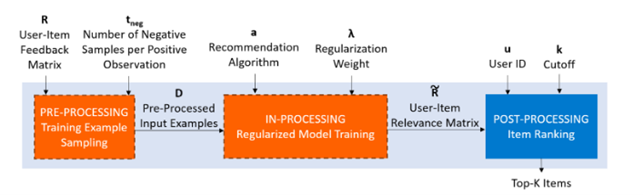
\includegraphics[]{pairwise_model.png}
	\caption[H διαδικασία μετριασμού της μεροληψίας που παρουσιάζεται στο ``Connecting user and item perspectives in popularity
	debiasing for collaborative recommendation", L. Boratto, G. Fenu, and M. Marras]{H διαδικασία μετριασμού της μεροληψίας που παρουσιάζεται στο ``Connecting user and item perspectives in popularity
		debiasing for collaborative recommendation", L. Boratto, G. Fenu, and M. Marras [Πηγή: \url{https://arxiv.org/pdf/2006.04275.pdf}]}
	\label{fig:pairwise}
\end{figure}
\noindent Στο \cite{borattoConnectingUserItem2021} παρουσιάζεται μια διαδικασία μετριασμού της μεροληψίας η οποία αποτελείται από τρία βήματα. Πρόκειται στην ουσία για τον συνδυασμό των τριών τεχνικών που προαναφέρθηκαν: pre-processing, in-processing και post-processing.\\
Η pre-processing τεχνική στο σενάριο βελτιστοποίησης ανά-ζεύγη (pair-wise optimization setting), για κάθε χρήστη u, δημιουργούνται t τριπλέτες (u, i, j) ανά παρατηρηθείσα αλληλεπίδραση χρήστη-αντικειμένου 
(u, i). To αντικείμενο j που δεν έχει παρατηρηθεί επιλέγεται ανάμεσα σε αντικείμενα λιγότερο δημοφιλή από το i, για t/2 παραδείγματα εκπαίδευσης (training examples), και μεταξύ των πιο δημοφιλών από το i για τα υπόλοιπα t/2 παραδείγματα. Με αυτόν τον τρόπο τα training examples αντιπροσωπεύουν ισότιμα τόσο τα δημοφιλή όσο και τα λιγότερο δημοφιλή αντικείμενα που σχετίζονται με το αντικείμενο που έχει παρατηρηθεί (observed item). Τα training examples συμβολίζονται με D.\\
Βασίζεται σε έναν pairwise αλγόριθμο, τον BPR και σε έναν pointwise, τον NeuMF. Στην in-processing τεχνική (\textit{Regularized Optimization (reg)}) o αλγόριθμος προσπαθεί να πετύχει ένα αντιστάθμισμα ανάμεσα στην ακρίβεια και στο popularity bias. Ο αρχικός αλγόριθμος λαμβάνει ως είσοδο το σύνολο εκπαίδευσης D χωρισμένο σε κομμάτια (batches), καθένα από αυτά τα κομμάτια συμβολίζεται με $ D_{batch} $, για να εκτελέσει μια επαναληπτική διαδικασία στοχαστικής καθόδου κλίσης (stochastic gradient descent). Η προσέγγιση που ακολουθείται όσον αφορά τη συνάρτηση βελτιστοποίησης βασίζεται στις αρχικές συναρτήσεις βελτιστοποίησης των pointwise και pairwise αλγορίθμων. Με αυτό το σκεπτικό ορίζεται η ακόλουθη συνάρτηση βελτιστοποίησης:
\begin{align}
	\min_\theta\left( 1-\lambda \right) \mathcal{L}\left( D_{batch} |\theta \right) + \lambda C\left( D_{batch} |\theta \right)
	\end{align}
Όπου $ λ \in\ [0,1] $ είναι το βάρος (weight) που εκφράζει το αντιστάθμισμα ανάμεσα στην απώλεια ακρίβειας (accuracy loss) και στην απώλεια κανονικοποίησης (regularization loss), δηλαδή στην μεροληψία που εισάγεται. Με $ λ=0 $ είναι σαφές πως δίνεται προτεραιότητα στην απώλεια ακρίβειας χωρίς να λαμβάνουμε υπόψη την απώλεια κανονικοποίησης. Αντίθετα, αν $ λ=1 $ δίνεται προτεραιότητα στην απώλεια κανονικοποίησης.
Με $ \mathcal{L} $ συμβολίζεται η συνάρτηση απώλειας ακρίβειας, η οποία εξαρτάται από την οικογένεια αλγορίθμων συστημάτων συστάσεων που χρησιμοποιείται. Ενώ με C συμβολίζεται η κανονικοποίηση  της συσχέτισης ανάμεσα στα προβλεφθέντα υπόλοιπα (predicted residuals) και στην παρατηρηθείσα δημοφιλία των αντικειμένων (observed item popularity).
Για τον υπολογισμό της συσχέτισης ανάμεσα στις κατανομές A1 και A2, χρησιμοποιείται η συνάρτηση Correlation:
\begin{align}
	C\left( D_{batch} |\theta \right) = | \text{Corrrelation}(A_1, A_2) |
\end{align}
όπου
\begin{align}
	A_1(b) = \mathcal{L}\left( D_{batch}(b) |\theta \right), \text{με} \  b \in \left\lbrace 0,\cdots,|D_{batch}| \right\rbrace 
	\end{align}
και:
\begin{align}
	A_2(b) = \frac{1}{\|U\|} \sum_{u \in U} \min\left(R(u,s), 1 \right)  \text{με} \ b \in \left\lbrace 0,\cdots,|D_{batch}| \right\rbrace 
\end{align}
Όπου $ R(u, s) $ το feedback που έδωσε ο χρήσης u για το αντικείμενο s στο σύνολο εκπαίδευσης. Όπως γίνεται αντιληπτό από τον ορισμό των δύο αυτών κατανομών, εάν η ικανότητα του μοντέλου να προβλέψει το εάν ένα αντικείμενο είναι αρκετά σχετικό εξαρτάται από τη δημοφιλία αυτού του αντικειμένου, τότε λαμβάνει κάποια «ποινή» μέσω της παραμέτρου λ.\\
Η post-processing τεχνική δεν παρουσιάζεται και αφήνεται στην ευχέρεια του χρήστη η επιλογή του κατάλληλου post-processing αλγορίθμου.